% fig_clique_interdiction: clique interdiction on a toy graph, and the
% certificate behind the new optima (3-partition + Mantel).
% Graph G: n = 8 vertices, m = 22 edges, leader budget k = 5 edges.
%   Groups V1 = {0,1,2}, V2 = {3,4,5}, V3 = {6,7}.
%   Edges inside groups: 01 12 34 45 67 (5).
%   Edges between groups: every pair except 07 23 15 46 (17).
%   omega(G) = 4.  Checked by brute force over all C(22,5) deletions:
% (a) Deleting 01 03 04 26 47 leaves exactly one largest clique, {1,3,6,7}
%     (size 4).
% (b) Deleting the 5 inside edges leaves a 3-partite graph, so no 4-clique:
%     omega <= 3.  Any 5 deletions leave 17 > floor(8^2/4) = 16 edges, so a
%     triangle survives (Mantel): omega >= 3.  The optimum is 3; e.g. the
%     triangle {1,3,6} survives the certificate deletion.
% Build: pdflatex fig_clique_interdiction.tex   (6.5 in x 2 in)
\documentclass[tikz,border=2pt]{standalone}
\pdfinfoomitdate=1 \pdftrailerid{} \pdfsuppressptexinfo=-1 % byte-identical rebuilds
\usepackage{mathptmx}
\usetikzlibrary{arrows.meta,calc,shapes.geometric}
\definecolor{leader}{HTML}{2A78D6}
\definecolor{follower}{HTML}{EB6834}
\definecolor{cert}{HTML}{1BAF7A}
\definecolor{ink}{HTML}{0B0B0B}
\definecolor{ink2}{HTML}{52514E}
\definecolor{muted}{HTML}{A9A8A2}
\definecolor{grid}{HTML}{E6E5E0}
\tikzset{
  every picture/.style={font=\fontsize{8}{9.6}\selectfont, color=ink, line cap=round},
  ptitle/.style={anchor=west, inner sep=0pt},
  small/.style={font=\fontsize{7}{8.4}\selectfont},
  vtx/.style={circle, draw=ink2, line width=0.7pt, fill=white, minimum size=0.27cm, inner sep=0pt},
  vsq/.style={rectangle, draw=ink2, line width=0.7pt, fill=white, minimum size=0.24cm, inner sep=0pt},
  vdi/.style={diamond, draw=ink2, line width=0.7pt, fill=white, minimum size=0.32cm, inner sep=0pt},
  hit/.style={draw=follower, fill=follower!45, line width=0.9pt},
  edge/.style={ink2, line width=0.55pt},
  deleted/.style={muted, line width=0.8pt, dash pattern=on 2.2pt off 1.6pt},
  clq/.style={follower, line width=1.6pt},
  grp/.style={draw=cert, line width=0.9pt, fill=cert!10, rounded corners=7pt},
}
% vertex positions on an ellipse, shared by both panels; each group sits on
% one arc: V1 = 0,1,2 (left), V2 = 3,4,5 (right), V3 = 6,7 (bottom)
\newcommand{\cx}{2.35}\newcommand{\cy}{2.2}
\newcommand{\rx}{2.0}\newcommand{\ry}{1.85}
\newcommand{\places}{%
  \foreach \i/\a in {0/112.5, 1/157.5, 2/202.5, 3/67.5, 4/22.5, 5/-22.5,
                     6/247.5, 7/292.5}
    \coordinate (p\i) at ({\cx+\rx*cos(\a)},{\cy+\ry*sin(\a)});}
% a deleted edge: dashed grey with a small grey cross at its midpoint
% (deleted/interdicted = grey with a cross, as in the other figures)
\newcommand{\xmark}[1]{%
  \draw[ink2, line width=0.7pt]
    ($#1+(-0.075,-0.075)$) -- ($#1+(0.075,0.075)$)
    ($#1+(-0.075,0.075)$) -- ($#1+(0.075,-0.075)$);}
% \deledge[pos]{u}{v}: the cross sits at fraction pos (default 0.5) along u-v
\newcommand{\deledge}[3][0.5]{%
  \draw[deleted] (p#2) -- (p#3);
  \fill[white] ($(p#2)!#1!(p#3)$) circle (0.11);
  \xmark{($(p#2)!#1!(p#3)$)}}
% a soft aqua band along the ellipse from angle #1 to #2 (one group)
\newcommand{\band}[2]{%
  \draw[cert!22, line width=0.62cm, line cap=round]
    plot[domain=#1:#2, samples=30, smooth, variable=\t]
    ({\cx+\rx*cos(\t)},{\cy+\ry*sin(\t)});}
\begin{document}
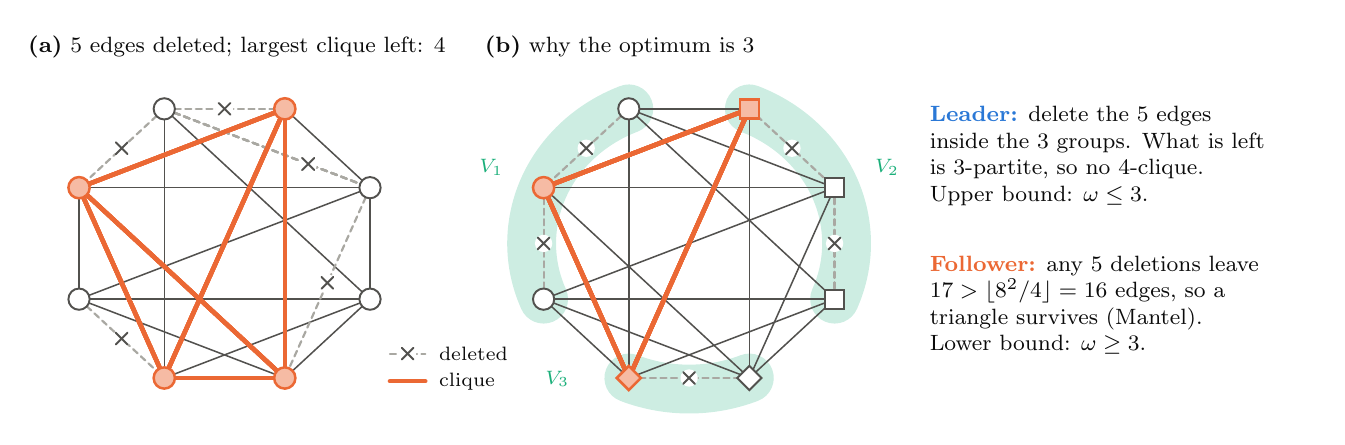
\begin{tikzpicture}
  % fixed page: 6.5 in x 2 in including the 2 pt border
  \useasboundingbox (0,0) rectangle (16.37,4.94);

  % ======================= (a) one leader move ==========================
  \begin{scope}[shift={(0.15,0)}]
    \places
    \node[ptitle] at (-0.15,4.70) {\textbf{(a)} 5 edges deleted; largest clique left: 4};
    % edges that stay (22 - 5 deleted)
    \foreach \u/\v in {1/2, 3/4, 4/5, 6/7,
                       0/5, 1/3, 1/4, 2/4, 2/5,
                       0/6, 1/6, 1/7, 2/7,
                       3/6, 3/7, 5/6, 5/7}
      \draw[edge] (p\u) -- (p\v);
    % the leader's 5 deletions
    \foreach \u/\v in {0/1, 0/3, 2/6, 4/7}
      \deledge{\u}{\v}
    \deledge[0.7]{0}{4} % its midpoint lies under the clique edge 3-6
    % the follower's largest clique {1,3,6,7}
    \foreach \u/\v in {1/3, 1/6, 1/7, 3/6, 3/7, 6/7}
      \draw[clq] (p\u) -- (p\v);
    \foreach \i in {0,2,4,5} \node[vtx] at (p\i) {};
    \foreach \i in {1,3,6,7} \node[vtx, hit] at (p\i) {};
    % key
    \draw[deleted] (4.45,0.80) -- ++(0.45,0);
    \fill[white] (4.675,0.80) circle (0.11);
    \xmark{(4.675,0.80)}
    \node[small, anchor=west] at (4.95,0.80) {deleted};
    \draw[clq] (4.45,0.45) -- ++(0.45,0);
    \node[small, anchor=west] at (4.95,0.45) {clique};
  \end{scope}

  % ======================= (b) the certificate ===========================
  \begin{scope}[shift={(6.05,0)}]
    \places
    \node[ptitle] at (-0.25,4.70) {\textbf{(b)} why the optimum is 3};
    % the three groups
    \band{112.5}{202.5}
    \band{-22.5}{67.5}
    \band{247.5}{292.5}
    \node[small, text=cert] at ({\cx+1.36*\rx*cos(157.5)},{\cy+1.36*\ry*sin(157.5)}) {$V_1$};
    \node[small, text=cert] at ({\cx+1.36*\rx*cos(22.5)},{\cy+1.36*\ry*sin(22.5)}) {$V_2$};
    \node[small, text=cert] at ({\cx+1.36*\rx*cos(232)},{\cy+1.18*\ry*sin(232)}) {$V_3$};
    % edges between groups stay
    \foreach \u/\v in {0/3, 0/4, 0/5, 1/3, 1/4, 2/4, 2/5,
                       0/6, 1/6, 1/7, 2/6, 2/7,
                       3/6, 3/7, 4/7, 5/6, 5/7}
      \draw[edge] (p\u) -- (p\v);
    % the 5 edges inside groups are deleted
    \foreach \u/\v in {0/1, 1/2, 3/4, 4/5, 6/7}
      \deledge{\u}{\v}
    % a triangle that survives
    \foreach \u/\v in {1/3, 1/6, 3/6}
      \draw[clq] (p\u) -- (p\v);
    \foreach \i in {0,2} \node[vtx] at (p\i) {};
    \node[vtx, hit] at (p1) {};
    \foreach \i in {4,5} \node[vsq] at (p\i) {};
    \node[vsq, hit] at (p3) {};
    \node[vdi] at (p7) {};
    \node[vdi, hit] at (p6) {};
  \end{scope}

  % the argument, in two lines each
  \begin{scope}[shift={(11.45,0)}]
    \node[anchor=north west, align=left, inner sep=0pt] at (0,3.95)
      {\textbf{\color{leader}Leader:} delete the 5 edges\\
       inside the 3 groups. What is left\\
       is 3-partite, so no 4-clique.\\
       Upper bound: $\omega \le 3$.};
    \node[anchor=north west, align=left, inner sep=0pt] at (0,2.05)
      {\textbf{\color{follower}Follower:} any 5 deletions leave\\
       $17 > \lfloor 8^2/4 \rfloor = 16$ edges, so a\\
       triangle survives (Mantel).\\
       Lower bound: $\omega \ge 3$.};
  \end{scope}
\end{tikzpicture}
\end{document}
